\chapter{相对论运动学}\label{ch:b3:relativistic-kinematics}

宇宙射线撞击高层大气，在距地面十五
千米处产生μ子——一种不稳定粒子，平均寿命为两
微秒。以接近光速运动，两微秒内飞行的距离是
六百米；然而海平面上的μ子探测器却持续计数，
所计数的粒子已穿越其允许射程的二十倍。
这一佯谬的解答并非粒子
物理的细节，而是对全部物理学基础概念的修正：时间
流逝对运动的μ子与对我们而言不同，距离
沿其运动方向收缩。本章由两条假设建立这一修正——狭义相对论
（爱因斯坦，1905 年），其两条假设为：物理定律
在每一惯性参考系中形式相同，真空中的光
在所有惯性参考系中具有相同速率。其余结论皆由严格的
运动学推出：洛伦兹变换中空间与时间的纠缠、
时间延缓、长度收缩、
新的速度叠加法则，以及几何——时空及其
不变间隔——在其中，这一切变得如同
转动一般自然。

\section{两条假设与绝对时间的冲突}

\begin{remark}[冲突从何而来]\label{rem:b3:relativistic-kinematics:conflict}
力学中早已有相对性原理：在平稳航行的船舱内，
任何用小球和单摆进行的实验都无法揭示船的运动
（伽利略）；牛顿定律在每一\emph{惯性
参考系}中都成立，所谓惯性参考系，是指彼此之间以恒定速度运动的参考系。
然而，本科二年级分册中的电磁学
导出了光速的确定值，$c = 1/\sqrt{\varepsilon_0\mu_0} =
\qty{3.00e8}{m/s}$，由自然常数决定，不涉及由谁来测量；
实验也与之相符：星光抵达
运动的地球，跨越四季所测得的光速从未改变
（迈克耳孙与莫雷，1887 年，以及此后所有的后继实验）。伽利略运动学
中速度可以相加，它无法容纳对所有人都相同的速率。
必须有所舍弃，问题出在我们所作的假设：
时间与同时性是绝对的。
\end{remark}

\begin{theorem}[狭义相对论的假设]\label{thm:b3:relativistic-kinematics:postulates}
\index{相对论!假设}\index{惯性参考系}
\emph{(i) 相对性：}物理定律在每一
惯性参考系中形式相同；任何实验都无法区分静止与匀速运动。
\emph{(ii) 光速：}真空中的光以相同速率 $c$
在每一惯性参考系中传播，无论光源或
观察者如何运动。
\end{theorem}
\admitted

\begin{definition}[事件与同时性]\label{def:b3:relativistic-kinematics:event}
\index{事件}\index{同时性}
\emph{事件}是一个点状的发生：有确定的位置\emph{和}确定的时刻——一次火花、
一次探测器计数、一次衰变。每一惯性
参考系为事件赋予坐标 $(t, x, y, z)$，所用的是在该参考系中
静止的尺子以及分布于其中且已同步的时钟。
两事件称为\emph{在某参考系中同时}，当该参考系的时钟
赋予它们相同的 $t$ 时——假设的第一个牺牲品，
正是这一概念依赖于参考系。
\end{definition}

\begin{example}[列车与两次闪电]\label{ex:b3:relativistic-kinematics:train}
闪电击中一列高速列车的两端，在列车
与轨道上留下痕迹。对于地面上位于两痕迹中点的观察者，
两道闪光同时到达：两次击中对她而言
是同时发生的。然而，坐在列车中点的乘客
正朝向其中一道闪光运动、远离另一道；他所在的参考系中光速同样为 $c$，
因此前方的闪光先到达他——既然他在
\emph{列车上}与两痕迹等距，他必须断定
前方的击中\emph{更早}发生。两种判断都没有错：
分离事件的同时性不是世界的事实，而是
参考系的性质。相对论中的每一个“佯谬”都在此消解。
\end{example}

\begin{omfigure}
\begin{tikzpicture}[font=\small, >=Stealth]
  % ground view
  \begin{scope}
    \draw[thick] (-0.3,0) -- (10.3,0);
    \fill[omDef!18, draw=omDef, thick, rounded corners=2pt] (1.4,0.15) rectangle (8.6,1.05);
    \foreach \x in {2.2,3.4,4.6,5.8,7.0} \draw[omDef] (\x,0.35) rectangle (\x+0.7,0.85);
    \draw[->, very thick] (8.9,0.6) -- (9.9,0.6) node[right] {$v$};
    \node[omExo] at (1.4,1.75) {\Large$\downarrow$};
    \node[omExo] at (8.6,1.75) {\Large$\downarrow$};
    \node[omExo, font=\footnotesize] at (1.4,2.15) {击中 A};
    \node[omExo, font=\footnotesize] at (8.6,2.15) {击中 B};
    \fill (5,-0.02) circle (2pt);
    \node[font=\footnotesize] at (5,-0.4) {地面观察者（中点）};
    \fill[omThm] (5,1.22) circle (2pt);
    \node[omThm, font=\footnotesize] at (5.1,1.55) {乘客（车厢中部）};
  \end{scope}
\end{tikzpicture}

{\small 两次击中标记了列车与轨道。地面观察者
位于两痕迹中点，同时接收两道闪光：对她而言两次击中同时发生。
乘客朝闪光 B 运动，闪光 B 先到达
他；他在自己的参考系中与两痕迹等距，
因此断定 B 先击中。同时性是相对的。}
\end{omfigure}

\section{洛伦兹变换}

\begin{theorem}[洛伦兹变换]\label{thm:b3:relativistic-kinematics:lorentz}
\index{洛伦兹变换}\index{伽马因子@$\gamma$ 因子}
设参考系 $\mathcal R'$ 以速度 $v$ 沿 $x$ 轴运动，
此轴属于参考系 $\mathcal R$，两者原点在 $t = t' = 0$ 时重合。
事件 $(t, x)$ 在 $\mathcal R$ 中，其在 $\mathcal R'$ 中的坐标为
\[
x' = \gamma\,(x - vt) , \qquad
t' = \gamma\Big(t - \frac{v\,x}{c^2}\Big) , \qquad
\gamma = \frac{1}{\sqrt{1 - v^2/c^2}} ,
\]
其中 $y' = y$，$z' = z$；逆变换与之形式相同，只需
将 $v \to -v$ 即可。当 $v \ll c$ 时，$\gamma \to 1$，即得伽利略
变换 $x' = x - vt$，$t' = t$。因子 $\gamma \ge 1$ ——
日常速度下几乎为 $1$，$1.15$（对应 $c/2$），$7.1$（对应 $0.99c$）——度量了
本章的每一种相对论效应。
\end{theorem}

\begin{proof}[部分证明]
时空的均匀性迫使变换为线性；
两参考系之间的对称性与相对性假设将其约化为
$x' = \gamma(x - vt)$，$x = \gamma(x' + vt')$，其中仅含一个未知
函数 $\gamma(v)$。考察从共同
原点发出的光闪：假设(ii)要求 $x = ct$ \emph{且} $x' = ct'$。
代入得 $ct' = \gamma t(c - v)$ 与 $ct = \gamma t'(c + v)$；
将两式相乘，得 $c^2 = \gamma^2(c^2 - v^2)$，
即所述的 $\gamma$。由两个线性关系消去 $x'$，
即得时间公式。（从“光速一致”到
“完整变换被确定”这一步——横向上无残余伸缩
或重标度——利用了
\cref{exo:b3:relativistic-kinematics:11}中详述的对称性论证。）
\end{proof}

\begin{proposition}[时间延缓]\label{prop:b3:relativistic-kinematics:dilation}
\index{时间延缓}\index{固有时}
在 $\mathcal R'$ 中静止（滴答位于 $x'$ 固定处）的时钟，
从 $\mathcal R$ 中观测时走得慢：其两次滴答之间相隔
的\emph{固有时} $\Delta\tau$（即时钟所在参考系中的时间），
参考系 $\mathcal R$ 测得
\[
\Delta t = \gamma\,\Delta\tau \ge \Delta\tau .
\]
运动的时钟走得慢——所有时钟皆然，无论是生物钟、原子钟，
还是亚原子钟，因为延缓的是时间本身，而非某种机制。
\end{proposition}

\begin{proof}
两次滴答位于同一 $x'$ 处：由逆变换得 $\Delta t
= \gamma(\Delta t' + v\,\Delta x'/c^2) = \gamma\,\Delta\tau$，因为
$\Delta x' = 0$。光钟图像
（\cref{exo:b3:relativistic-kinematics:2}）给出同样的 $\gamma$，
仅由毕达哥拉斯定理即可得到。
\end{proof}

\begin{proposition}[长度收缩]\label{prop:b3:relativistic-kinematics:contraction}
\index{长度收缩}\index{固有长度}
\emph{固有长度}为 $L_0$ 的杆（即其在静止参考系中的长度），
沿长度方向以速率 $v$ 运动，在实验室中测得
\[
L = \frac{L_0}{\gamma} \le L_0 .
\]
横向尺度不变。测量运动的杆，意味着
在\emph{实验室的同一时刻}确定其两端的位置——而
同时性依赖于参考系，因此长度也依赖于参考系。
\end{proposition}

\begin{proof}
在实验室同一时刻 $t$ 标记两端：由变换得
$\Delta x' = \gamma(\Delta x - v\Delta t) = \gamma\,\Delta x$，其中
$\Delta t = 0$，且 $\Delta x' = L_0$，于是 $\Delta x = L_0/\gamma$。
\end{proof}

\begin{omfigure}
\begin{tikzpicture}[font=\small, >=Stealth]
  % light clock at rest
  \begin{scope}
    \draw[thick] (-0.7,0) -- (0.7,0);
    \draw[thick] (-0.7,2.2) -- (0.7,2.2);
    \draw[->, omExo, thick] (0,0.08) -- (0,2.12);
    \node[anchor=west] at (0.12,1.1) {$c\,\Delta\tau$};
    \node at (0,-0.55) {静止的光钟：一次滴答};
  \end{scope}
  % moving light clock
  \begin{scope}[xshift=5.6cm]
    \draw[thick] (-0.7,0) -- (4.7,0);
    \draw[thick] (-0.7,2.2) -- (4.7,2.2);
    \draw[gray, dashed] (0,0) -- (0,2.2);
    \draw[gray, dashed] (4,0) -- (4,2.2);
    \draw[->, omExo, thick] (0,0.08) -- (1.96,2.12);
    \draw[->, omExo, thick] (2.04,2.12) -- (4,0.14);
    \node[rotate=47, anchor=south] at (0.85,1.0) {$c\,\Delta t/2$};
    \draw[->, thick] (0,-0.35) -- (4,-0.35);
    \node at (2,-0.75) {镜子向前移动 $v\,\Delta t$};
    \node at (2,3.0) {$\Big(\dfrac{c\Delta t}{2}\Big)^2 = \Big(\dfrac{v\Delta t}{2}\Big)^2 + \Big(\dfrac{c\Delta\tau}{2}\Big)^2$};
  \end{scope}
\end{tikzpicture}

{\small 光钟：一个光子在两面镜子之间来回反射。从
光钟运动的参考系看去，光子沿更长的
斜线路径、以相同速率 $c$ 传播：滴答所需时间更长，
$\Delta t = \gamma\,\Delta\tau$，仅由毕达哥拉斯定理即得。}
\end{omfigure}

\begin{example}[μ子的两种解释]\label{ex:b3:relativistic-kinematics:muon}
一个μ子的速率为 $v = 0.995c$，其 $\gamma = 10$。在我们的参考系中，
它的内部时钟慢了十倍：其两微秒的固有寿命被拉长
为二十微秒，它飞行了六千米，而不是六百米。
在μ子自身的参考系中，其寿命仍是普通的 \qty{2.2}{\micro s}——
但迎面冲来的山脉被压缩为原来的十分之一，恰好能容纳其中。
两个参考系都认同同一个物理事实，即\emph{μ子是否到达探测器}：
相对论改变的是时间和长度，从不改变
结果（\cref{pb:b3:relativistic-kinematics:1}）。
\end{example}

\begin{method}[理清各种效应]\label{met:b3:relativistic-kinematics:method}
(1) 确定\emph{事件}（发射、到达、滴答、衰变），而非
“物体”。(2) 固有时 $\Delta\tau$ 属于同时经历两个事件的那一个时钟：
其他参考系测得的时间更长，
为 $\gamma\Delta\tau$。(3) 固有长度 $L_0$ 属于杆的静止参考系：
其他参考系测得的长度更短，为 $L_0/\gamma$。(4) 出现
“佯谬”时，找出那两个在空间上分离的事件，
它们被悄悄当作同时发生的，并追问：在哪个参考系中？(5) 检验
极限 $v/c \to 0$，并记住 $\gamma - 1 \approx \tfrac12 v^2/c^2$，
在低速下——正是日常相对论修正的量级。
\end{method}

\section{速度的合成；多普勒效应}

\begin{proposition}[相对论速度合成]\label{prop:b3:relativistic-kinematics:addition}
\index{速度合成}
若物体以 $u'$ 沿 $x'$ 方向在参考系 $\mathcal R'$ 中运动，
而该参考系本身以 $v$ 相对 $\mathcal R$ 运动，
则 $\mathcal R$ 测得的速度不是 $u' + v$，而是
\[
u = \frac{u' + v}{1 + u'v/c^2} .
\]
日常速率下分母为 $1$，于是回到伽利略的结果；当
$u' = c$ 时，公式给出 $u = c$，无论 $v$ 为何值——光对所有人都以 $c$ 传播，
这是理论内置的要求；任何低于 $c$ 的速度合成都不可能
达到 $c$。
\end{proposition}

\begin{proof}
$u = \dd x/\dd t$，由逆变换：$\dd x =
\gamma(\dd x' + v\,\dd t')$，$\dd t = \gamma(\dd t' + v\,\dd x'/c^2)$；
相除即得。
\end{proof}

\begin{example}[菲涅耳系数的解释]\label{ex:b3:relativistic-kinematics:fizeau}
静水中的光速为 $c/n$。在以 $v$ 流动的水中，菲佐
于 1851 年测得令人费解的 $c/n + v(1 - 1/n^2)$，而非完全拖曳的
$c/n + v$。将 $u' = c/n$ 与 $v$ 合成：
\[
u = \frac{c/n + v}{1 + v/nc}
\approx \Big(\frac{c}{n} + v\Big)\Big(1 - \frac{v}{nc}\Big)
\approx \frac{c}{n} + v\Big(1 - \frac{1}{n^2}\Big) ,
\]
精确到 $v/c$ 的一阶。这一十九世纪的台面实验结果，
在当时无法解释，实际上是速度合成定律的一阶近似——
爱因斯坦于 1905 年援引的诸多无声证实之一。
\end{example}

\begin{proposition}[纵向多普勒效应]\label{prop:b3:relativistic-kinematics:doppler}
\index{多普勒效应!相对论}
固有频率为 $f_0$ 的波源沿视线以速率 $v = \beta c$ 远离时，
接收频率为
\[
f = f_0\,\sqrt{\frac{1 - \beta}{1 + \beta}}
\qquad
\text{（接近时：} \beta \to -\beta\text{）} .
\]
两种效应相叠加：其一是经典的到达时间拉长，
因为每个波峰出发时都离接收者更远；其二是相对论性的波源钟变慢——
这里的 $\gamma$ 即使在 $90^\circ$ 方向上仍然存在（
\emph{横向}多普勒效应，纯粹是时间延缓）。
\end{proposition}

\begin{proof}
在接收者参考系中，波源每隔
$\gamma/f_0$（时间延缓）发出一个波峰，每个波峰比前一个多走 $v\gamma/f_0$ 的距离，因此
波峰每隔 $\gamma(1 + \beta)/f_0 = \sqrt{(1+\beta)/
(1-\beta)}\,/f_0$ 到达一次。
\end{proof}

\begin{example}[星系的退行]\label{ex:b3:relativistic-kinematics:redshift}
氢谱线发出时波长为 \qty{656.3}{nm}，
而来自遥远星系的接收波长为 \qty{689}{nm}：$f/f_0 = 0.953$，故 $\beta \approx 0.048$——
该星系以 \qty{14000}{km/s} 的速率退行。将这一公式用于整个天空，
仅此一个公式便将光谱变成了膨胀宇宙的图景；
本书最后一章将继续这一故事。
\end{example}

\section{时空与时空间隔}

\begin{theorem}[不变时空间隔]\label{thm:b3:relativistic-kinematics:interval}
\index{时空}\index{时空间隔}
对任意两个事件，组合
\[
\Delta s^2 = c^2\,\Delta t^2 - \Delta x^2 - \Delta y^2 - \Delta z^2
\]
在每个惯性参考系中取值都相同——这是相对论在时间与长度发生伸缩时
所保持不变的量。其符号对事件对作如下分类：
\emph{类时}（$\Delta s^2 > 0$）：存在某个参考系使两事件位于同一地点，
且 $\Delta s/c$ 为二者之间的固有时；
\emph{类空}（$\Delta s^2 < 0$）：存在某个参考系使两事件同时发生，
且二者之间不可能有信号相连；\emph{类光}
（$\Delta s^2 = 0$）：只有光能将二者相连。
\end{theorem}

\begin{proof}
直接代入洛伦兹变换：
$c^2t'^2 - x'^2 = \gamma^2\big[(ct - \beta x)^2 - (x - \beta ct)^2
\big] = \gamma^2(1 - \beta^2)(c^2t^2 - x^2) = c^2t^2 - x^2$。
关于分类：使两事件位于同一地点，需要一个
速率为 $v = \Delta x/\Delta t$ 的参考系，当 $|\Delta x| <
c\,|\Delta t|$（类时）时可以实现；使两事件同时发生，则需要 $v =
c^2\Delta t/\Delta x$ 的参考系，当 $|\Delta x| > c\,|\Delta t|$
（类空）时可以实现。
\end{proof}

\begin{remark}[因果性有其几何]\label{rem:b3:relativistic-kinematics:causality}
\index{光锥}
过每个事件都有其\emph{光锥}：它能影响的事件（未来锥），
能影响它的事件（过去锥）——
以及因果上被切断的类空“其他处”。由于
类空事件对的先后次序依赖于参考系——有的参考系看到 A 先于 B，
另一些看到 B 先于 A——任何超光速信号都会让某个
观察者看到结果先于原因。相对论的速度上限
并非关乎发动机，而是保持历史自洽的代价。
\end{remark}

\begin{omfigure}
\begin{tikzpicture}[font=\small, >=Stealth, scale=0.92]
  % axes
  \draw[->] (-3.6,0) -- (3.9,0) node[right] {$x$};
  \draw[->] (0,-2.6) -- (0,3.4) node[above] {$ct$};
  % light cone
  \fill[omExo!14] (0,0) -- (2.9,2.9) -- (-2.9,2.9) -- cycle;
  \fill[omExo!14] (0,0) -- (2.4,-2.4) -- (-2.4,-2.4) -- cycle;
  \draw[omExo, thick] (-2.9,-2.9) -- (2.9,2.9);
  \draw[omExo, thick] (2.9,-2.9) -- (-2.9,2.9);
  \node[omExo, font=\footnotesize, anchor=west] at (2.6,2.35) {光，$x = ct$};
  \node[font=\footnotesize] at (-0.55,2.35) {未来};
  \node[font=\footnotesize] at (0,-2.1) {过去};
  \node[font=\footnotesize] at (3.05,0.7) {其他处};
  \node[font=\footnotesize] at (-3.0,0.7) {其他处};
  % worldline
  \draw[omDef, very thick] (-0.9,-2.5) .. controls (0.2,-0.6) and (-0.5,1.2) .. (0.75,3.1);
  \node[omDef, font=\footnotesize, anchor=west] at (0.85,3.25) {世界线};
  % event
  \fill (0,0) circle (2pt);
\end{tikzpicture}

{\small 围绕一个事件（原点处的点）的时空。其光锥划分出它能够影响的
区域（未来）、可能影响它的区域（过去），以及
类空的其他区域。物质世界线陡于 $45^\circ$
——始终处于光锥之内。}
\end{omfigure}

\begin{example}[远行的孪生子]\label{ex:b3:relativistic-kinematics:twins}
一个孪生子飞往距离 $8$ 光年的恒星，
速度为 $0.8c$（$\gamma = 5/3$），往返一次。地球上的时间：$2 \times 8/0.8 =
\qty{20}{yr}$。旅行者的固有时：$20/\gamma = \qty{12}{yr}$
——旅行者年轻八年，并无佯谬：两位孪生子的处境
\emph{并不}对称，因为其中一条世界线是直的（全程为惯性的），
另一条在折返处有一个折角。在两个固定
事件之间，直线世界线是固有时\emph{最长}的那一条；
——在时空几何中，绕行路径的固有时更短。这一
效应已被常规测量：环绕地球飞行的原子钟
与留在地面的同类钟相比，读数恰好相差预言的
纳秒数（\cref{pb:b3:relativistic-kinematics:1}）。
\end{example}

\begin{omfigure}
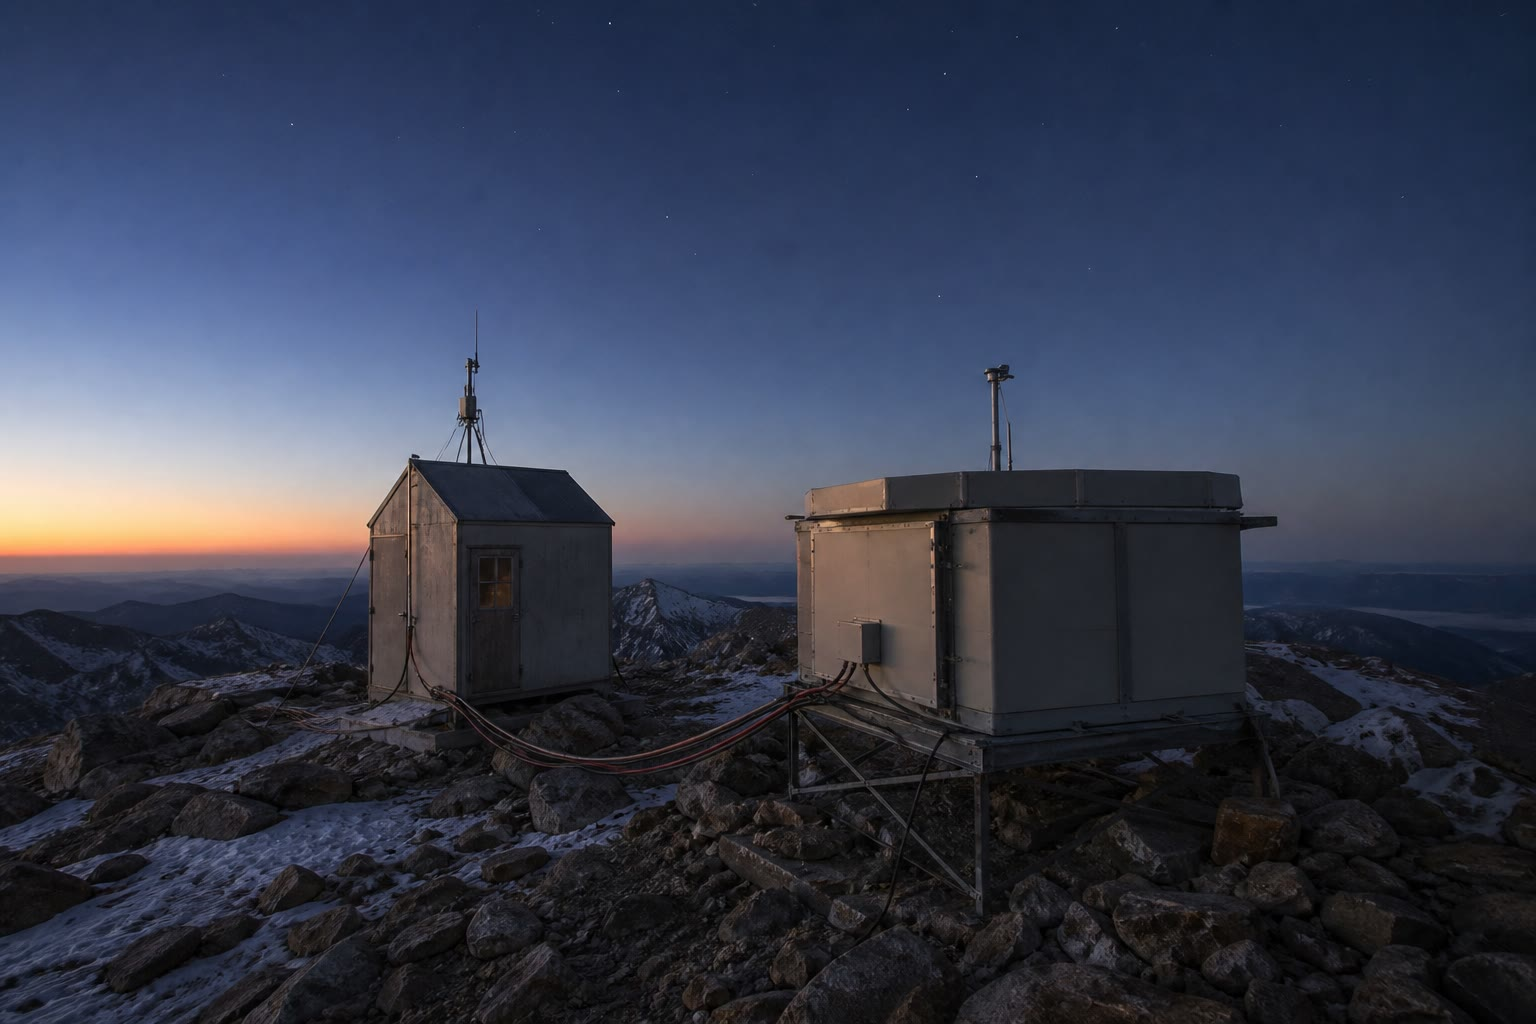
\includegraphics[width=0.58\linewidth]{images/book5/ai/b5-04-cosmic-ray-station.jpg}

{\small 高海拔处的宇宙射线观测站。它所计数的μ子在高出十千米处产生，只因运动的钟走得慢，它们才能到达这里——时间延缓效应每晚都在山顶上得到测量。}
\end{omfigure}

\section{练习}

\begin{exercise}[$\star$]\label{exo:b3:relativistic-kinematics:1}
求 $\gamma$，其中 $v/c = 0.1$、$0.5$、$0.9$、$0.99$、$0.999$。对于
国际空间站（\qty{7.7}{km/s}），用小速度近似计算 $\gamma - 1$，
以及乘组在每个六个月任务中相对于地面时钟“获得”（或损失？）的时间，
相对于地面上的时钟，
并忽略引力。
\end{exercise}

\begin{exercise}[$\star$]\label{exo:b3:relativistic-kinematics:2}
图中的光钟：（a）写出静止光钟的一次滴答时间 $\Delta\tau =
2d/c$（$d$ 为两镜面间距）；（b）
在钟以 $v$ 运动的参考系中，由毕达哥拉斯定理推出 $\Delta t =
\gamma\Delta\tau$；（c）为何该论证要求两参考系中的横向距离
$d$ 相同？（d）用两把相同的尺相互经过的论证，
说明横向长度
不会改变。
\end{exercise}

\begin{exercise}[$\star$]\label{exo:b3:relativistic-kinematics:3}
一个μ子在 \qty{15}{km} 高度处产生，速度 $v = 0.999c$。（a）其
$\gamma$ 及在我们参考系中的平均寿命。（b）它所经过的平均距离。
（c）在其自身参考系中大气层的厚度。（d）
这类μ子中有多大比例能到达地面，分别计入与不计入相对论（衰变律
$\eu^{-t/\tau}$，$\tau = \qty{2.2}{\micro s}$）？
\end{exercise}

\begin{exercise}[$\star$]\label{exo:b3:relativistic-kinematics:4}
$x$ 轴上的两个事件：A 位于 $(t = 0, x = 0)$，B 位于 $(t =
\qty{2}{\micro s}, x = \qty{300}{m})$。（a）计算 $\Delta s^2$：
是类时还是类空？（b）A 能否导致 B？（c）求使 A 与 B 发生在同一地点的参考系的速率，
以及它们之间的
固有时。（d）对 B 位于
$(\qty{1}{\micro s}, \qty{600}{m})$ 的情形，提出同样的三个问题——哪一个参考系
现在存在，哪一个不存在？
\end{exercise}

\begin{exercise}[$\star\star$]\label{exo:b3:relativistic-kinematics:5}
GPS 卫星沿轨道运行，速度 $v = \qty{3.87}{km/s}$。（a）计算 $\gamma -
1$。（b）卫星钟每天比地面钟慢多少，
仅由时间延缓引起？（c）定位依靠以
$c$ 传播的信号计时：若不作修正，一天内由狭义相对论漂移引起的
位置误差相当于多少？（d）完整的修正（计入引力，
按末章的思路处理）为 $+38\,\unit{\micro s}$，
每天，引力蓝移\emph{占上风}，压过了时间延缓：
这一符号告诉你，在 
\qty{20200}{km} 高度处，哪一效应更大？
\end{exercise}

\begin{exercise}[$\star\star$]\label{exo:b3:relativistic-kinematics:6}
（a）一艘飞船以 $0.8c$ 飞行，相对于自身以 $0.8c$ 向前发射一个
探测器，求其相对我们的速率？（b）两艘飞船相向运动，
在我们的参考系中各以 $0.9c$ 运动，二者的相对速率为多少？（c）由速度合成律证明
若 $u' < c$ 且 $v < c$，则可推出 $u < c$（对
表达式 $c - u$ 作因式分解）。（d）用激光笔扫过
月面，光斑可以以超过 $c$ 的速度移动：为何这并不违背
任何定律？
\end{exercise}

\begin{exercise}[$\star\star$]\label{exo:b3:relativistic-kinematics:7}
来自一颗恒星的钠双线，其静止波长为 \qty{589.0}{nm}，到达时
波长为 \qty{575.0}{nm}。（a）是靠近还是远离？速率为多少？（b）
多大速率下，可见光（\qty{550}{nm}）会被移到
近红外（\qty{1100}{nm}）？（c）对 $\beta \ll 1$，证明
$\Delta\lambda/\lambda \approx \beta$，并给出经验法则：在 \qty{600}{nm} 处，
每 \unit{\angstrom} 对应的速率（km/s）。（d）一个以恒定距离绕行的源
即使没有径向运动也显示频移：这是哪种效应，
它是 $\beta$ 的几阶量？
\end{exercise}

\begin{exercise}[$\star\star$]\label{exo:b3:relativistic-kinematics:8}
撑杆与谷仓。一根 \qty{20}{m} 长的撑杆以 $\gamma = 2$ 运动，
携带着冲向一个 \qty{10}{m} 长、带两扇门的谷仓。（a）撑杆在谷仓参考系中的
长度是多少，它能装进谷仓吗？（b）在跑者参考系中，\emph{谷仓}的长度为
\qty{5}{m}，两种结论怎能都正确？标出两个事件
（“前门关闭”、“后门打开”），并比较它们在两个参考系中的时间顺序。
（c）计算在谷仓中同时关门的情形下，这些事件在
每个参考系中的时间间隔。（d）
用一句话概括寓意（“佯谬”隐含了哪一条未言明的假设？）。
\end{exercise}

\begin{exercise}[$\star\star$]\label{exo:b3:relativistic-kinematics:9}
一枚固有长度为 \qty{100}{m} 的火箭，以
$0.6c$ 的速度掠过空间站。（a）空间站的钟从火箭机头
经过到机尾经过，历时多久？（b）对于火箭上的钟，观测
空间站（固有长度为 \qty{300}{m}）经过，同样的问题如何？（c）
在其参考系中同时发射两个对接夹钳，
相距 \qty{80}{m}：对火箭而言，两次发射之间的时间间隔为多少，
哪一个先发射？（d）验证这对夹钳事件的 $\Delta s^2$ 在两个参考系间
相同。
\end{exercise}

\begin{exercise}[$\star\star\star$]\label{exo:b3:relativistic-kinematics:10}
双生子全题。斯特拉以 $0.8c$ 的速度飞往一颗恒星，
该恒星距地球 \qty{8}{ly}（地球参考系），她再以 $0.8c$ 的速度返回；特拉留在地球上。（a）计算
两人各自经历的时间。（b）在斯特拉去程的参考系中，恒星有多远？
去程历时多久？（c）刚好在掉头之前和之后，
斯特拉对“地球上此刻的时间”的计算结果分别是多少
（利用 $vx/c^2$ 项）？说明她的时间账在转折处跳变了若干年，
并说明这一跳变恰好使两人的总时间相互吻合。（d）
解释为什么不能从斯特拉一侧进行
对称的论证。
\end{exercise}

\begin{exercise}[$\star\star\star$]\label{exo:b3:relativistic-kinematics:11}
洛伦兹变换的诚实推导。（a）由齐次性论证
变换必须是线性的。（b）假设 $x' = \gamma(x - vt)$，并由
相对性原理得 $x = \gamma(x' + vt')$，推导 $t'$，
用 $t$ 和 $x$ 表示，且不借助光。（c）证明要求
$x = ct \Rightarrow x' = ct'$ 时，$\gamma$ 恰好取其给定的值。（d）
论证中究竟在何处用到了每一条假设？
\end{exercise}

\begin{exercise}[$\star\star\star$]\label{exo:b3:relativistic-kinematics:12}
快度。定义 $\varphi$，使 $\tanh\varphi = \beta$。（a）证明
洛伦兹变换可写为 $ct' = ct\cosh\varphi - x\sinh\varphi$，
$x' = x\cosh\varphi - ct\sinh\varphi$：一个“旋转”，其旋转角为虚数，
它保持 $c^2t^2 - x^2$ 不变，正如旋转保持 $x^2 + y^2$ 不变。
（b）证明速度的合成\emph{使快度相加}：$\varphi =
\varphi_1 + \varphi_2$，并由
$\tanh(\varphi_1 + \varphi_2)$ 导出速度合成公式。（c）一枚火箭在自身参考系中以 $g$ 的加速度加速；
承认其快度按 $\dd\varphi = g\,
\dd\tau/c$ 增长，求 $\beta(\tau)$，以及
它达到 $0.99c$ 所需的固有时。（d）为什么快度可以无限增长，
而 $\beta$ 不能？
\end{exercise}

\begin{omfigure}
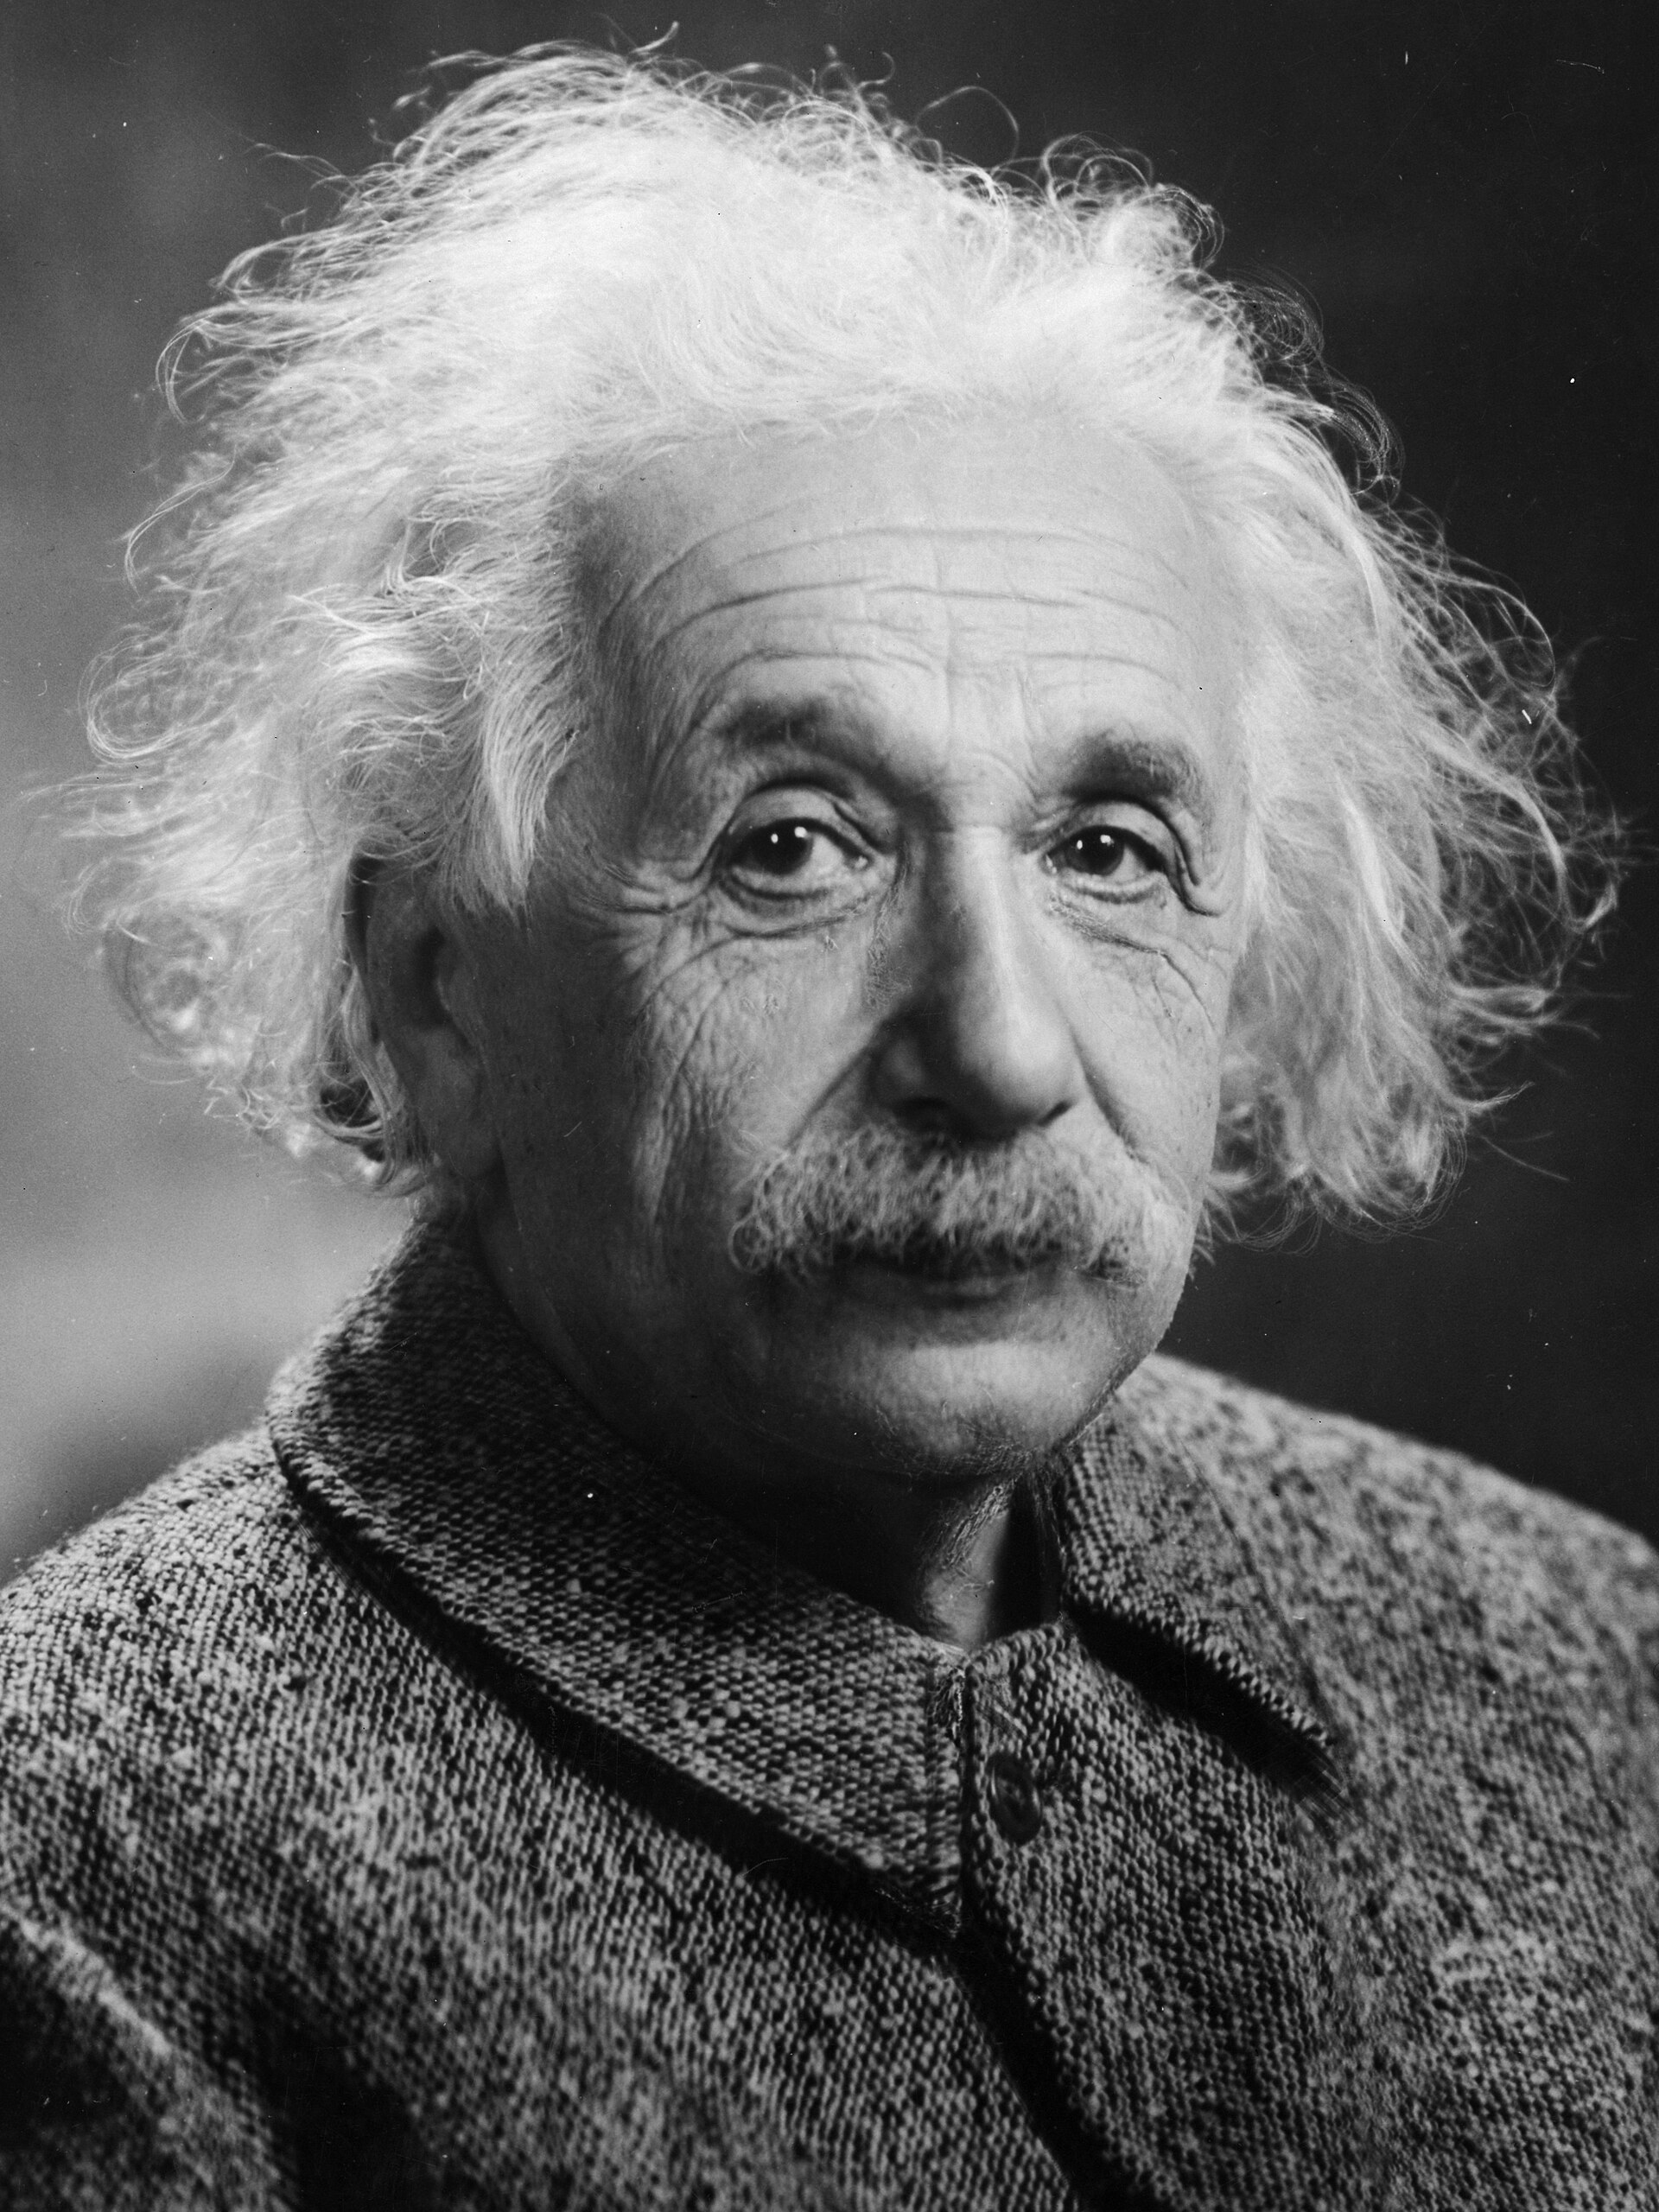
\includegraphics[width=0.34\linewidth]{images/book5/photo-einstein-1947.jpg}

{\small 爱因斯坦（照片：Orren Jack Turner，1947 年，公有领域）。1905 年的相对论论文从两条假设重建了运动学——本章基本保持该论文的内容，并增加了练习。}
\end{omfigure}

\section{问题：天空中的实验}

\begin{problem}[{周末问题——μ 子、山上的钟与时间延缓的
证明}]\label{pb:b3:relativistic-kinematics:1}
最干净的早期时间延缓检验不需要任何实验装置：
大自然成千上万地提供相对论性的钟，
它们从每座山的上空落下。本题重现弗里施–史密斯
实验（1963 年），然后把同样的物理推广到客机和
导航卫星。数据：μ 子的平均固有寿命 $\tau =
\qty{2.20}{\micro s}$；衰变服从指数规律，
$\eu^{-t/\tau}$ 即 μ 子经固有时 $t$ 后的存活比例；$c =
\qty{3.00e8}{m/s}$；华盛顿山两探测器之间的海拔差 $h =
\qty{1907}{m}$。

\medskip\noindent\textbf{第一部分——从天而降的钟。}
\begin{enumerate}
  \item 宇宙质子在高层大气中撞击原子核，碎片
        在约 \qty{15}{km} 高处衰变为 μ 子。为什么一群相同的不稳定粒子
        可以作为\emph{钟}？
  \item 计算 $c\tau$，即 μ 子平均寿命对应的自然射程。
  \item 若不考虑相对论，在
        \qty{15}{km} 高处产生、并以基本为 $c$ 的速度运动的 μ 子，有多大比例能到达
        地面？（写出指数；数值本身
        荒谬。）
  \item 海平面的探测器能大量计数到 μ 子：用一句话
        指出其中的矛盾。
  \item 海平面的通量约为每平方厘米每分钟一个 μ 子：
        估算每秒有多少 μ 子穿过你伸出的手，
        以及两次心跳之间有多少 μ 子穿过你的身体。
  \item 实验选取速率为 $0.995c$ 的 μ 子：计算
        它们的 $\gamma$。
  \item 弗里施和史密斯每小时计得 $563 \pm 10$ 个 μ 子，
        在山顶测得。为什么要在\emph{同一}簇射的两个海拔处测量，
        而不是直接相信 \qty{15}{km} 处的产生图像？
\end{enumerate}

\medskip\noindent\textbf{第二部分——山上的测量。}
\begin{enumerate}[resume]
  \item 以 $0.995c$ 的速度走完 \qty{1907}{m} 的行程，
        在山的参考系中需要多长时间？
  \item 若不考虑时间延缓，有多大比例的 μ 子能穿过这段行程？
        底部探测器每小时应计得多少个？
  \item 考虑时间延缓后，μ 子在此行程中经历的\emph{固有}时间
        为多少？
  \item 利用相对论，预测
        存活比例与每小时的计数。
  \item 测得底部每小时的计数为 $408 \pm 9$。将
        两种预测与数据比较，并指出哪一种理论
        经受住了山的检验。
  \item 由测得的比值 $408/563$，求出
        \emph{实验}时间延缓因子，并与
        $\gamma = 10$ 比较。（μ 子在类岩石屏蔽层中
        略有减速，因此有效的 $\gamma$ 略低于
        山顶处的数值——弗里施和史密斯得到 $8.8 \pm
        0.8$。）
\end{enumerate}

\medskip\noindent\textbf{第三部分——μ 子自身的故事。}
\begin{enumerate}[resume]
  \item 在 μ 子的参考系中，华盛顿山有多高？
  \item 山从它身边掠过需要多长时间？在此时间内
        有多大比例的 μ 子发生衰变？检验其与
        第二部分的预测一致。
  \item 两个参考系对何者被延缓的看法不一（是我们的时间？\ 还是
        山？），却对计数取得一致：计数属于哪一类量，
        为什么所有参考系都必须对它取得一致？
  \item 计算从山顶产生到底部到达之间的
        时空间隔 $\Delta s^2$（在山的参考系中），并检验
        $\Delta s/c$ 等于第二部分中 μ 子的固有时间。
  \item 一位怀疑者反驳说：“也许改变衰变速率的是海拔，
        而不是速度。”测得的 $\gamma$ 依赖关系
        （速度较慢的 μ 子延缓较少）提供了怎样的对照？
  \item 现代存储环将 μ 子保持在 $\gamma = 29.3$，
        寿命测至 $\num{e-3}$ 的精度：它们发现了什么，
        圆周轨道又为这一检验增加了什么（哪一个孪生子是
        μ 子？）
\end{enumerate}

\medskip\noindent\textbf{第四部分——回到地面：飞机与
卫星。}
\begin{enumerate}[resume]
  \item 一架客机以 \qty{250}{m/s} 的速度巡航，完成
        历时 \qty{40}{h} 的环球飞行。利用 $\gamma - 1 \approx v^2/2c^2$，
        计算其时钟的狭义相对论性滞后量，
        单位为纳秒。
  \item 铯钟很容易分辨纳秒量级；1971 年的飞行
        证实了该预测（计入引力的反向作用，
        高空处更强，已计入）。为什么必须
        \emph{向东和向西都飞}，才能把两种效应分离开？
  \item 一颗 GPS 卫星（$v = \qty{3.87}{km/s}$）每天累积的
        狭义相对论性时钟滞后量为多少微秒？
  \item 若不加修正，这种漂移
        仅\emph{一周}便会产生多少千米的测距误差？
  \item GPS 的完整修正量为每天 $+38\,\unit{\micro s}$
        （包括引力效应），已在发射前植入卫星时钟：
        若不做这一修正，导航员
        在数小时内会观测到什么？
  \item 概括这一命名结果：一座山、两台计数器和
        $2.2\,\unit{\micro s}$ 的钟于 1963 年测得时间延缓，
        $\gamma \approx 9$ 时误差在 $10\%$ 以内——而同样的
        物理，如今在每一部手机中每秒都被修正，
        这些手机都知道自身所在的位置。
\end{enumerate}
\end{problem}
